
\section{Lecture 8: Conjugate gradients and Krylov subspaces}
\sectionlabel{TBD}
These lecture notes describe approaches to solving non-convex problems with a particular focus on Krylov subspaces, Chebyshev polynomials, and the conjuagte gradient method.
\subsection{Krylov subspaces}
Finding the eigenvalues of a matrix is a standard non-convex problem. Below we list the standard methods for solving linear equations and for solving eigenvalue equations. 
\begin{center}
\begin{tabular}{ | c |c| c | } 
\hline
 & $Ax=b$ & $Ax=\lambda x$ (non convex) \\ 
\hline
Basic & Gradient descent & Power methods \\ 
\hline
Accelerated & Chebyshev iteration & Chebyshev iteration \\
\hline
Accelerated and step size free & Conjugate gradient & Lanczos \\
\hline
\end{tabular}
\end{center}
\begin{remark}[Chebyshev]
The Chebyshev iteration requires step sizes to be carefully chosen while the ``accelerated and step size free'' methods do not.
\end{remark}
\begin{definition}[Krylov subspace]
For a matrix $A \in \R^{n x n}$ and a vector $b \in \R^n$, 
the Krylov sequence of order $t$ is $b, Ab, A^2b, ...., A^tb$. We define the Krylov subspace as the $\mathrm{span}\{b, Ab, A^2b, \ldots, A^t\} \subseteq \R^n$. 
\end{definition}
\begin{fact}[Polynomial connection]
If $A$ has eigenvectors $u_1, ... u_n$ and $t \geq \mathrm{rank}{A}$ and $\langle b,u_i\rangle \neq 0$, then $u_i \in K_t \ \forall i$
\end{fact}


Suppose we have a vector $v \in K_t(A,b)$, this implies:
\begin{align*}
v \in K_t(A,b) &\Longleftrightarrow \exists \alpha_i: \ v= \alpha_0 b + \alpha_1 Ab + \cdots \alpha_t A^tb
\end{align*}
If we define $p(A) \sum_{i=1}^t \alpha_i A^i$ then $v = p(A)b$. Then $K_t(A,b) = \left\{ p(A)b : \text{deg}(p) \leq t \right\}$. \\

Suppose we have a symmetric matrix $A \in \R^{n \times n}$ that has orthonormal eigenvectors $u_1 \ldots u_n$ and ordered eigenvalues $\lambda_1 \geq \lambda_2 \ldots \geq \lambda_n$. Now suppose we write $b$ in this basis, $b=\alpha_1 u_1 + ... + \alpha_n u_n$ with $\alpha_i = \langle u_i,b\rangle$. 
\begin{remark}[Orthonormal eigenvectors]
\begin{align*}
    \langle u_i,u_j\rangle &= 0, \ i \neq j \\
    \langle u_i, u_i\rangle &= 1 
\end{align*}
\end{remark}

\begin{remark}
$p(A)u_i = p(\lambda_i)u_i$
\end{remark}
Subsequently:
\begin{align*}
A &= \sum \lambda_i u_i \trspvec{u_i}  \\
p(A) &= \sum p(\lambda_i) u_i \trspvec{u_i} \\
 p(A)b &= \alpha_1 p(\lambda_1)u_1 + \alpha_2 p(\lambda_2) u_2 + \ldots + \alpha_n p(\lambda_n) u_n 
\end{align*}
 
We want to find a polynomial such that $p(A)b \approx \alpha_1 u_1$. Ideally, we would have $ p(\lambda_1) = 1$ and $ p(\lambda_i) = 0 \ \text{for } i > 1$. One way to achieve this goal is to get $p(\lambda_1) = 1$ and $\max{p(\lambda_i)}_{i>1}$ as small as possible. This will give us a close approximation to the top eigenvalue. \\

We consider the following ``easy'' polynomial that will get us pretty close to this goal:
\begin{align*}
    p(\lambda) &= \frac{\lambda^t}{\lambda_1 ^t} \\
    \text{From this we get:} \\
    p(\lambda_1) &= 1 \\
    p(\lambda_2) &= (\frac{\lambda_2}{\lambda_1})^t
\end{align*}
We want $p(\lambda_2)$ to get small so we are interested in how close $\lambda_2$ is to $\lambda_1$. Consider 
$\lambda_1 = (1 + \epsilon) \lambda_2$ then we need $p(\lambda_2) = \frac{1}{(1+\epsilon)^t}$ if we want $p(\lambda_2)$ to become small. 
\begin{remark}[$\angle$ notation]
$\tan \angle (a,b)$ is the tangent of the angle between $a$ and $b$
\end{remark}
\begin{theorem}[]
$\tan \angle(p(A)b, u_1) \leq \max_{j>1} \frac{|p(\lambda_j)|}{|p(\lambda_1)|} \tan \angle (b, u)$
\end{theorem}


\begin{proof}
We define $\theta = \angle (u_1,b)$. By this, we get
\begin{align*}
    \sin ^2 \theta &=  \sum_{j >1} \alpha_j^2 \\
    \cos ^2 \theta &= |\alpha_1|^2 \\
    tan^2 \theta &= \sum_{j \rangle 1} \frac{|\alpha_j^2|}{|\alpha_1|^2}
\end{align*}
Now we can write:
\begin{align*}
    \tan^2 \angle (p(A)b, u_1) = \sum_{j>1} \frac{|p(\lambda_j)\alpha_j|^2}{|p(\lambda_1)\alpha_1|^2} \leq \underset{j\rangle1}{\text{max}} \frac{|p(\lambda_j)|^2}{|p(\lambda_1)|^2} \sum_{j\rangle1} \frac{\alpha_j |^2}{|\alpha_1| ^2}
\end{align*}
We note that this last sum $ \sum_{j > 1} \frac{\alpha_j |^2}{|\alpha_1| ^2}= \tan \theta$ and we obtain our desired result.
\end{proof}
We apply this to $p(\lambda) = \frac{\lambda^t}{\lambda_1^t}$ and $\lambda_1 = (1+\epsilon) \lambda_2$. This implies $\tan \angle(p(A)b, u_1) \leq \frac{1}{(1+\epsilon)t} \tan \angle(u_1, b)$. If there is a big gap between $\lambda_1$ and $\lambda_2$ this converges quickly but it can be slow if $\lambda_1 \approx \lambda_2$.

\begin{definition}[Power method]
\begin{align*}
x_0 &= \frac{b}{\|b\|} \\
x_t &= \frac{A x_{t-1}}{\|Ax_{t-1}\|}
\end{align*}
\end{definition}
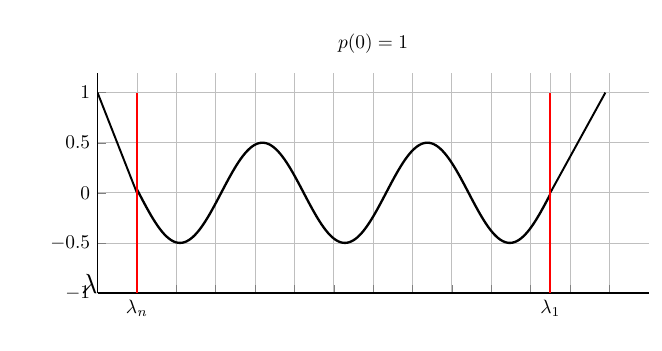
\begin{tikzpicture}[scale = 0.7]
  %\begin{axis}[doma
  in= 2:8,xlabel=$\lambda$,label style={font=\large},tick label style={font=\large}, ylabel style={yshift=-.1cm}, xmin=0, xmax=13, ymin=-1, ymax=1.5, xtick={}, ytick={-1, 0,1},trig format plots=rad,grid=both,grid style={dashed,gray}]
        \begin{axis}[%
                width=10cm,
                height=4cm,
                scale only axis,
                xmin=0, xmax=7,
                xtick={0.5, 1, 1.5,2, 2.5,3, 3.5,4, 4.5, 5, 5.5, 5.75, 6,6.5},
                xticklabels={$\lambda_n$,,,,,,,,,,,$\lambda_1$},
                xmajorgrids,
                ymin=-1, ymax=1.2,
                ymajorgrids,
                title={$p(0) = 1$},
                axis lines*=left,
                line width=1.0pt,
                mark size=2.0pt,
                legend style={at={(1.03,1)},anchor=north west,draw=black,fill=white,align=left}];
                \addplot[domain = 0.5:5.75, black, very thick,samples=200] {.5*(cos(3*deg(x) ))};
                \addplot[domain = 0:2] coordinates {(0,1)(0.5,0)};
                \addplot[domain = 6.17:8.3] coordinates {(5.75,0)(6.45,1)};
                \addplot[red] coordinates{(0.5,1)(0.5,-1)};
                \addplot[red] coordinates{(5.75,1)(5.75,-1)};
              
               
\end{axis}
\end{tikzpicture}
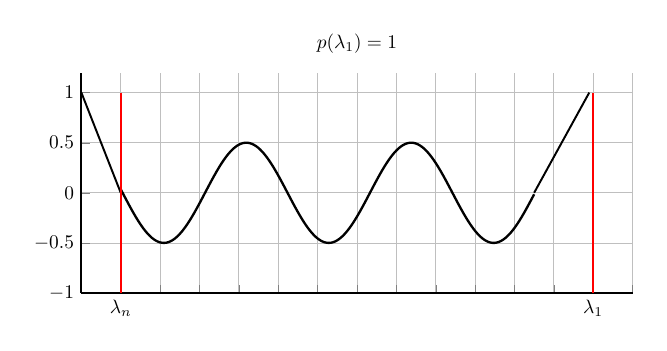
\begin{tikzpicture}[scale = 0.7]
        \begin{axis}[%
                width=10cm,
                height=4cm,
                scale only axis,
                xmin=0, xmax=7,
                xtick={0.5, 1, 1.5,2, 2.5,3, 3.5,4, 4.5, 5, 5.5, 6,6.5,7},
                xticklabels={$\lambda_n$,,,,,,,,,,,,$\lambda_1$},
                xmajorgrids,
                ymin=-1, ymax=1.2,
                ymajorgrids,
                title={$p(\lambda_1) = 1$},
                axis lines*=left,
                line width=1.0pt,
                mark size=2.0pt,
                legend style={at={(1.03,1)},anchor=north west,draw=black,fill=white,align=left}];
                \addplot[domain = 0.5:5.75, black, very thick,samples=200] {.5*(cos(3*deg(x) ))};
                \addplot[domain = 0:2] coordinates {(0,1)(0.5,0)};
                \addplot[domain = 6.17:8.3] coordinates {(5.75,0)(6.45,1)};
                \addplot[red] coordinates{(0.5,1)(0.5,-1)};
                \addplot[red] coordinates{(6.5,1)(6.5,-1)};
              
               
\end{axis}
\end{tikzpicture}
\subsection{Applying Chebyshev polynomials}
As in prior lectures, we need to normalize our Chebyshev polynomials. However, now we want to ensure that $p(\lambda_1) = 1$ so that we are picking out the first eigenvalue with the correct scaling. 

\begin{lemma}
A suitably rescaled degree $t$ Chebyshev polynomial achieves 
\begin{equation*}
\min_{p(\lambda_1)=1} \max_{\lambda \in [\lambda_2, \lambda_n]} p(\lambda) \leq \frac{2}{(1+\sqrt{\epsilon})^t}
\end{equation*}
where $\epsilon = \frac{\lambda_1}{\lambda_2} - 1$
\end{lemma}

\begin{center}
\begin{tabular}{ | c |c| c | } 
\hline
 & $Ax=b$ & $Ax=\lambda x$ (non convex) \\ 
\hline
$\epsilon$ & $\frac{1}{\kappa} = \frac{\alpha}{\beta}$ & $\frac{\lambda_1}{\lambda_2} -1$ \\ 
\hline
\end{tabular}
\end{center}

\subsection{Conjugate gradient method}
\begin{definition}[Algorithm for conjugate gradient]
We want to solve $Ax = b, \ A \geq 0$. 
\begin{align*}
x_0 &= 0: \text{ "solution"} \\
r_0 &= b: \text{ "residual"} \\
p_0 &= r_0: \text{ "search direction"} \\
\end{align*}
For t = 1,2, ....
\begin{align*}
\eta_t &= \frac{\|r_t\|}{\langlep_{t-1}, Ap_{t-1}\rangle}: \text{ "step size"} \\
x_t &= x_{t-1} + \eta_t p_{t-1} \\
r_t &= r_{t-1} - \eta_t A r_{t-1} \\
p_t &= r_t + \frac{\|r_t\|^2}{\|r_{t-1}^2\|}P_{t-1} \\ 
\end{align*}
\end{definition}

\begin{proof}
Proof by induction (see Trefethen and Bau). Show that conditions in Lemma \ref{lem:conjGrad} are true initially and stay true when the update rule is applied.  
\end{proof}
\begin{lemma}\label{lem:conjGrad}
The following three equations must always be true for the conjugate gradient method algorithm.
\begin{align*}
\mathrom{span}{\langle r_0, ...r_{t-1}\rangle} &= K_t(A,b) \\
j\langle t \ \langler_t, r_j\rangle &= 0, \ r_t \perp K_t(a,b) \\
i \neq j: \ p_i^{\trans} A p_j &= 0 \text{: "Conjugacy"} 
\end{align*}
\end{lemma}

\begin{lemma}
Let $\|u\|_A = \sqrt{\trspvec{u} A u}$ and $\langle u,v\rangle_A = \trspvec{u} A v$ and $e_t = x^* - x_t$. Then $e_t$ minimizes $\|x^* - x\|_A$ over all vectors $x \in K_{t-1}$.
\end{lemma}

\begin{proof}
We know that $x_t \in K_{t-1}$. Let $x \in K_{t-1}$ and define $x = x_t + \delta$. Then $e = x^* - x = x_t + \delta$. We compute the error in the $A$ norm.
\begin{align*}
\|x^* - x\|_A^2 &= \|e_t + \delta\|^{\trans} A(e_t + \delta) \\
e &= x^* - x \\
e &= x^* - x = e_t + \delta \\ 
\|x^* - x\|_A^2 &= e_t^{\trans}Ae_t + \delta^{\trans}A\delta + 2e_t^{\trans} A \delta \\
A\delta \in K_{t-1}
\end{align*}
We argue that the last term $2e_t^{\trans} A \delta = 0$ because $e_t$ is orthogonal to the Krylov subspace. By definition $e_t^{\trans}A = r_t$.
\end{proof}
